\documentclass{article}
\usepackage{hyperref} % For clickable links

\usepackage{ragged2e} % For justified text alignment
\usepackage{longtable}
\usepackage{booktabs} % For better table lines
\setlength{\parindent}{0pt} % Remove paragraph indentation
\usepackage{booktabs}
% Language setting
% Replace `english' with e.g. `spanish' to change the document language
\usepackage[english]{babel}
\usepackage{float} % To use [H] placement
% Set page size and margins
% Replace `letterpaper' with `a4paper' for UK/EU standard size
\usepackage[letterpaper,top=2cm,bottom=2cm,left=3cm,right=3cm,marginparwidth=1.75cm]{geometry}

% Useful packages
\usepackage{amsmath}
\usepackage{graphicx}

\usepackage{adjustbox} % To handle long rows
% \usepackage[colorlinks=true, allcolors=blue]{hyperref}

\onecolumn
\title{A Case of Study for Classification Algorithms Applied to a Tabular Vector-Borne Disease Dataset}
\author{Alberto Arath Figueroa Salomon}
\begin{document}
\maketitle

\section{Introduction}

Vector-borne diseases have become a major concern due to human activity that creates imbalances
in ecosystems. These diseases, transmitted through the bites of blood-sucking arthropods, have
become a recurring issue in warm climates. They share common features, including similar symptoms,
which can be nearly indistinguishable from one another.

The purpose of this study is to build a machine learning model capable of discerning classification
patterns based on these shared symptoms.

\section{Data}

\subsection{Instance Composition}

The dataset consists of labeled data with 707 rows and 64 features. The training data has a synthetic origin, so no additional data preparation is required. This allows us to focus solely on applying machine learning techniques.

% Table environment

\begin{table}[h!] % Single-column table
\centering
\renewcommand{\arraystretch}{1.2} % Adjust row spacing slightly
\scalebox{0.8}{ % Scale to 80% including caption
\begin{tabular}{|c|c|c|c|}
\hline
\textbf{Muscle Pain} & \textbf{Fatigue} & \textbf{Weakness} & \textbf{Prognosis} \\ \hline
Present              & Not Present      & Present           & Present            \\ \hline
Not Present          & Not Present      & Present           & Present            \\ \hline
\end{tabular}
} % End of scaling
\caption{Sample training set with a subset of features.}
\label{tab:sample_training}
\end{table}

\subsection{Predictor Set}

The predictor set consists of binary variables indicating whether a given symptom is present
in the prognosis instance. These binary variables represent the presence or absence of a specific
condition. The variable \( X \) takes values from the set:
\[
X \in \{0, 1\},
\]
where:
\[
X =
\begin{cases}
1 & \text{if the condition is \textbf{present}}, \\
0 & \text{if the condition is \textbf{not present}}.
\end{cases}
\]

\subsection{Target Variable}

The target variable, called Prognosis, represents the vector-borne disease classifier. The target
variable, denoted as \( Y \), is categorical and takes values from the following set of classes:
\[
Y \in \{ C_1, C_2, \dots, C_k \},
\] 
where \( C_i \) represents the \( i^{\text{th}} \) class label, for \( i = 1, 2, \dots, k \).

In this study, \( k = 11 \), and the classes are defined as follows:
\begin{itemize}
    \item \( C_1 \): Dengue,
    \item \( C_2 \): Zika,
    \item \( C_3 \): Malaria.
\end{itemize}
To apply machine learning algorithms, we use label encoding as follows:
\[
Y = 
\begin{cases} 
0 & \text{if the class is \( C_1 \) (Malaria)}, \\
1 & \text{if the class is \( C_2 \) (Dengue)}, \\
2 & \text{if the class is \( C_3 \) (Zika)}.
\end{cases}
\]
This encoding allows for the application of machine learning algorithms such as softmax regression, decision trees, or neural networks to predict the likelihood of each class based on the input features.

\section{Exploratory Data Analysis (EDA)}

\subsection{Class Distribution}

The class distribution shows no significant imbalance, as shown in Figure 1. West Nile Fever has 80
instances, while Malaria has 50. Although class imbalance could have an impact, we expect it to be
non-significant. For the sake of this study, we will apply oversampling techniques to improve the model.

\begin{figure*}[t] % Fix the figure at its exact position
    \centering
    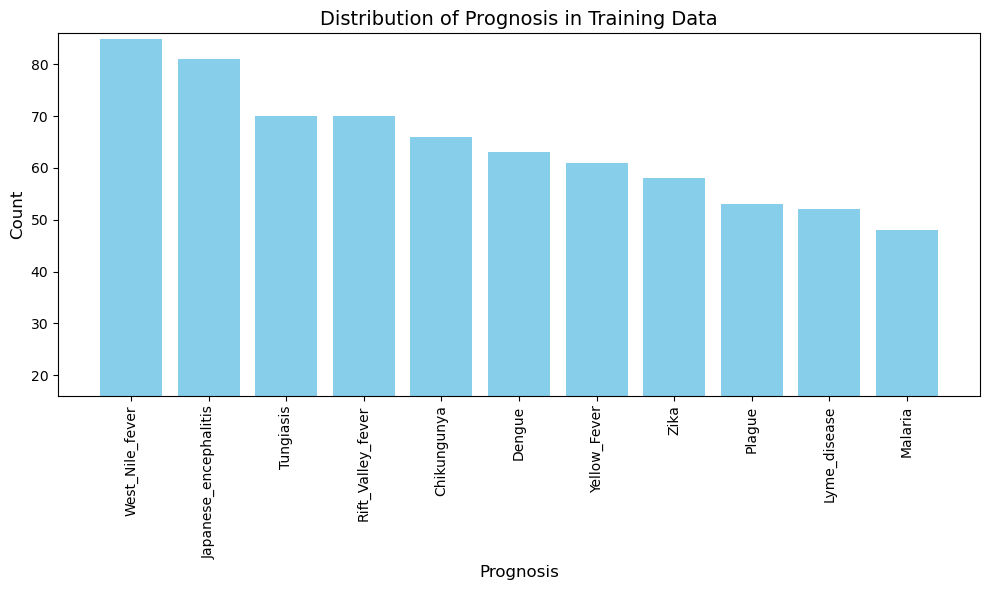
\includegraphics[width=.8\linewidth]{DiseaseDistribution.png}
    \caption{Distribution of Prognosis in Training Data.}
    \label{fig:disease_distribution}
    \vspace{-1em} % Reduce vertical spacing after the figure
\end{figure*}

\subsection{Feature Correlation Matrix}

The correlation matrix shows little correlation between features, suggesting that dimensionality
reduction techniques may not be effective. We will test this hypothesis in the modeling section.

\begin{figure}[H]  
\centering
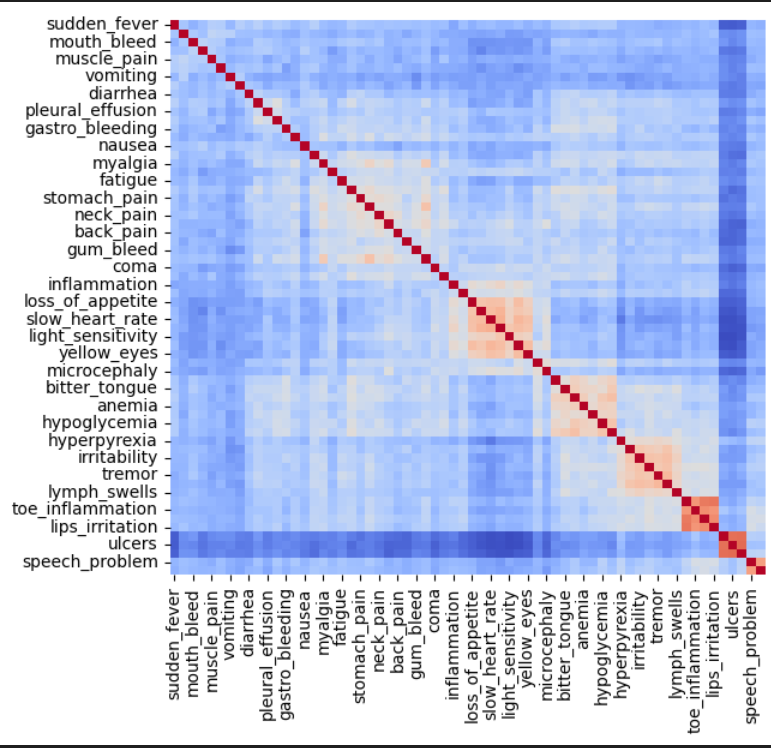
\includegraphics[width=1\linewidth]{CorrelationMatrix.png}
\caption{Features Correlation Heat Map. Blue areas indicate low correlation.}
\vspace{-1em} % Reduce vertical spacing
\end{figure}

\section{Methodology}

In this study, we performed hyperparameter tuning using Grid Search and evaluated several machine
learning algorithms to identify the best-performing model. The following algorithms were evaluated:

\subsection{Cross-Algorithms Grid Search Approach}

The metric used to evaluate the models is the precision metric. Other metrics, such as false negatives,
are outside the scope of this study.
\[
\text{Precision} = \frac{\text{True Positives (TP)}}{\text{True Positives (TP)} + \text{False Positives (FP)}}
\]

\subsection{Model Selection and Study}

The study will collect results for four algorithms and benchmark the scores based on different techniques
to improve model performance. A nested grid search will be applied, with the outer loop being the algorithm
under test and the inner loop defined by the hyperparameters of the given algorithm.

We will not explain the inner workings of the models, as this is outside the scope of the study.

\subsection{Hyperparameter Tuning}

Grid search was expanded by fixing all hyperparameters and gradually increasing the chosen hyperparameter.

\begin{itemize}
    \item Parameters used for each algorithm.
    \item Explanation of the performance results for each algorithm.
    \item Engineer's decision for selecting the best model for this dataset.
\end{itemize}

\subsection{K-Nearest Neighbors (KNN)}

The \textbf{K-Nearest Neighbors (KNN)} algorithm is a non-parametric, instance-based learning method.
It classifies a data point based on the majority class of its \(k\) nearest neighbors in the feature space.
Hyperparameters tuned include:
\begin{itemize}
    \item \textbf{n\_neighbors}: Number of neighbors considered.
    \item \textbf{weights}: Weighting function for neighbors (\textit{uniform} or \textit{distance}).
\end{itemize}

\begin{table}[bhtp]
    \centering
    \caption{KNeighborsClassifier Grid Search Results}
    \label{tab:table}
    \begin{tabular}{ccc}
    \toprule
    \textbf{mean\_test\_score} & \textbf{rank\_global\_score} & \textbf{classifier and hyperparameters} \\
    \midrule
    0.230935 & 11 & KNeighborsClassifier, n\_neighbors=7, weights='uniform' \\
    0.219302 & 14 & KNeighborsClassifier, n\_neighbors=5, weights='uniform' \\
    0.214970 & 18 & KNeighborsClassifier, n\_neighbors=7, weights='distance' \\
    0.200214 & 22 & KNeighborsClassifier, n\_neighbors=5, weights='distance' \\
    0.121799 & 27 & KNeighborsClassifier, n\_neighbors=3, weights='distance' \\
    0.121095 & 28 & KNeighborsClassifier, n\_neighbors=3, weights='uniform' \\
    \bottomrule
    \end{tabular}
\end{table}
    
\subsection{Random Forest Classifier}

The \textbf{Random Forest Classifier} is an ensemble learning method that constructs a collection of
decision trees and combines their predictions. It reduces overfitting compared to individual trees.
Hyperparameters tuned include:
\begin{itemize}
    \item \textbf{n\_estimators}: Number of trees in the forest.
    \item \textbf{max\_depth}: Maximum depth of each tree.
    \item \textbf{min\_samples\_split}: Minimum number of samples required to split an internal node.
\end{itemize}

\begin{table}[!htbp]
    \centering
    \caption{Random Forest Grid Search Results}
    \label{tab:table}
    \adjustbox{max width=\textwidth}{%
    \begin{tabular}{cccp{8cm}}
    \toprule
    \textbf{mean\_test\_score} & \textbf{rank\_test\_score} & \textbf{classifier} & \textbf{hyperparam\_combination} \\
    \midrule
    0.277801 & 1  & RandomForestClassifier & RandomForestClassifier, max\_depth=5, min\_samples\_split=2, n\_estimators=50 \\
    0.256374 & 3  & RandomForestClassifier & RandomForestClassifier, max\_depth=5, min\_samples\_split=2, n\_estimators=100 \\
    0.251517 & 4  & RandomForestClassifier & RandomForestClassifier, max\_depth=None, min\_samples\_split=2, n\_estimators=100 \\
    0.244632 & 5  & RandomForestClassifier & RandomForestClassifier, max\_depth=None, min\_samples\_split=5, n\_estimators=100 \\
    0.239188 & 8  & RandomForestClassifier & RandomForestClassifier, max\_depth=5, min\_samples\_split=5, n\_estimators=100 \\
    0.213390 & 19 & RandomForestClassifier & RandomForestClassifier, max\_depth=10, min\_samples\_split=5, n\_estimators=50 \\
    0.210364 & 20 & RandomForestClassifier & RandomForestClassifier, max\_depth=None, min\_samples\_split=5, n\_estimators=50 \\
    0.207067 & 21 & RandomForestClassifier & RandomForestClassifier, max\_depth=10, min\_samples\_split=2, n\_estimators=50 \\
    0.193830 & 23 & RandomForestClassifier & RandomForestClassifier, max\_depth=5, min\_samples\_split=5, n\_estimators=50 \\
    0.192695 & 24 & RandomForestClassifier & RandomForestClassifier, max\_depth=10, min\_samples\_split=2, n\_estimators=100 \\
    0.190548 & 25 & RandomForestClassifier & RandomForestClassifier, max\_depth=None, min\_samples\_split=2, n\_estimators=50 \\
    0.166299 & 26 & RandomForestClassifier & RandomForestClassifier, max\_depth=10, min\_samples\_split=5, n\_estimators=100 \\
    \bottomrule
    \end{tabular}%
    }
\end{table}


\subsection{Support Vector Classifier (SVC)}
The \textbf{Support Vector Classifier (SVC)} is a kernel-based method that finds an optimal hyperplane to separate classes in a high-dimensional space. Hyperparameters tuned include:
\begin{itemize}
    \item \textbf{C}: Regularization parameter.
    \item \textbf{kernel}: Kernel function (\textit{linear}, \textit{rbf}, or \textit{poly})  \textit{rbf} was just included 
    just for benchmark as it is widely used kernel
\end{itemize}

\begin{table}[!htbp]
    \centering
    \caption{SVC Grid Search Results}
    \label{tab:table}
    \adjustbox{max width=\textwidth}{%
    \begin{tabular}{cccp{7cm}}
    \toprule
    \textbf{mean\_test\_score} & \textbf{rank\_test\_score} & \textbf{classifier} & \textbf{hyperparam\_combination} \\
    \midrule
    0.276434 & 2  & SVC & SVC, C=0.1, kernel='linear' \\
    0.243171 & 6  & SVC & SVC, C=1, kernel='rbf' \\
    0.235429 & 10 & SVC & SVC, C=10, kernel='rbf' \\
    0.215171 & 16 & SVC & SVC, C=10, kernel='linear' \\
    0.215171 & 16 & SVC & SVC, C=1, kernel='linear' \\
    0.007571 & 29 & SVC & SVC, C=0.1, kernel='rbf' \\
    \bottomrule
    \end{tabular}%
    }
\end{table}
    

\subsection{Logistic Regression}
The \textbf{Logistic Regression} model is a linear classifier used for binary and multi-class classification problems. It models the probability of a class using the logistic function. Hyperparameters tuned include:
\begin{itemize}
    \item \textbf{penalty}: Type of regularization (\textit{l1}, \textit{l2}, or \textit{elasticnet}).
    \item \textbf{C}: Inverse of regularization strength.
    \item \textbf{solver}: Optimization algorithm for model fitting.
\end{itemize}

\begin{table}[!htbp]
    \centering
    \caption{Logistic Regression Grid Search Results}
    \label{tab:table}
    \adjustbox{max width=\textwidth}{%
    \begin{tabular}{ccp{8cm}} % Centered columns, with wrapped text for hyperparameters
    \toprule
    \textbf{mean\_test\_score} & \textbf{rank\_test\_score} & \textbf{hyperparam\_combination} \\
    \midrule
    0.242251 & 4  & maxiter=500, multiclass='ovr', solver='saga', C=10, penalty='l1' \\
    0.240382 & 5  & maxiter=500, multiclass='ovr', solver='saga', C=1, penalty='l1' \\
    0.238665 & 7  & maxiter=500, multiclass='ovr', solver='saga', C=0.1, penalty='l2' \\
    0.226524 & 13 & maxiter=500, multiclass='ovr', solver='saga', C=1, penalty='l2' \\
    0.216889 & 17 & maxiter=500, multiclass='ovr', solver='saga', C=10, penalty='l2' \\
    0.006944 & 30 & maxiter=500, multiclass='ovr', solver='saga', C=0.1, penalty='l1' \\
    \bottomrule
    \end{tabular}%
    }
\end{table}

\subsection {Best cross validation score training set}
Test set best cross validation Score 

\begin{table}[h!]
    \centering
    \caption{Classifier Results with Rank and Scores}
    \label{tab:classifier_ranks}
    \begin{tabular}{lcc}
    \toprule
    \textbf{Classifier}       & \textbf{Mean Test Score} & \textbf{Rank} \\
    \midrule
    KNeighborsClassifier      & 0.295575                & 1 \\
    RandomForestClassifier    & 0.293805                & 2 \\
    RandomForestClassifier    & 0.290265                & 3 \\
    KNeighborsClassifier      & 0.290265                & 4 \\
    RandomForestClassifier    & 0.288496                & 5 \\
    \bottomrule
    \end{tabular}
    \end{table}


\section{Results}

\begin{table}[H]
    \centering
    \caption{Training Set best results}
    \label{tab:hyperparam_table2}
    \adjustbox{max width=\textwidth}{%
    \begin{tabular}{ccp{8cm}}
    \toprule
    \textbf{mean\_test\_score} & \textbf{rank\_test\_score} & \textbf{hyperparam\_combination} \\
    \midrule
    0.304661 & 1 & RandomForestClassifier, max\_depth=10, min\_samples\_split=5, n\_estimators=100 \\
    0.295298 & 2 & RandomForestClassifier, max\_depth=10, min\_samples\_split=2, n\_estimators=50 \\
    0.292155 & 3 & RandomForestClassifier, max\_depth=None, min\_samples\_split=5, n\_estimators=100 \\
    0.288419 & 4 & SVC, C=10, kernel='rbf' \\
    0.283026 & 5 & SVC, C=1, kernel='rbf' \\
    \bottomrule
    \end{tabular}%
    }
\end{table}
    
\begin{table}[H]
    \centering
    \caption{Test Set best results}
    \label{tab:hyperparam_table1}
    \adjustbox{max width=\textwidth}{%
    \begin{tabular}{ccp{8cm}}
    \toprule
    \textbf{mean\_test\_score} & \textbf{rank\_test\_score} & \textbf{hyperparam\_combination} \\
    \midrule
    0.276434 & 1 & SVC, C=0.1, kernel='linear' \\
    0.251400 & 2 & RandomForestClassifier, max\_depth=10, min\_samples\_split=2, n\_estimators=100 \\
    0.246152 & 3 & RandomForestClassifier, max\_depth=10, min\_samples\_split=5, n\_estimators=100 \\
    0.243171 & 4 & SVC, C=1, kernel='rbf' \\
    0.242251 & 5 & LogisticRegression, maxiter=500, multiclass='ovr', solver='saga', C=10, penalty='l1' \\
    \bottomrule
    \end{tabular}%
    }
\end{table}
\subsection{Confusion Matrix}

The matrix shows significant confusions among classes that have similar symptom sets. For example:
"Japanese Encephalitis" and "Lyme Disease" have off-diagonal misclassifications.
"Tungiasis" has the strongest performance with 12 correct predictions.

\begin{figure}[H]  
    \centering
    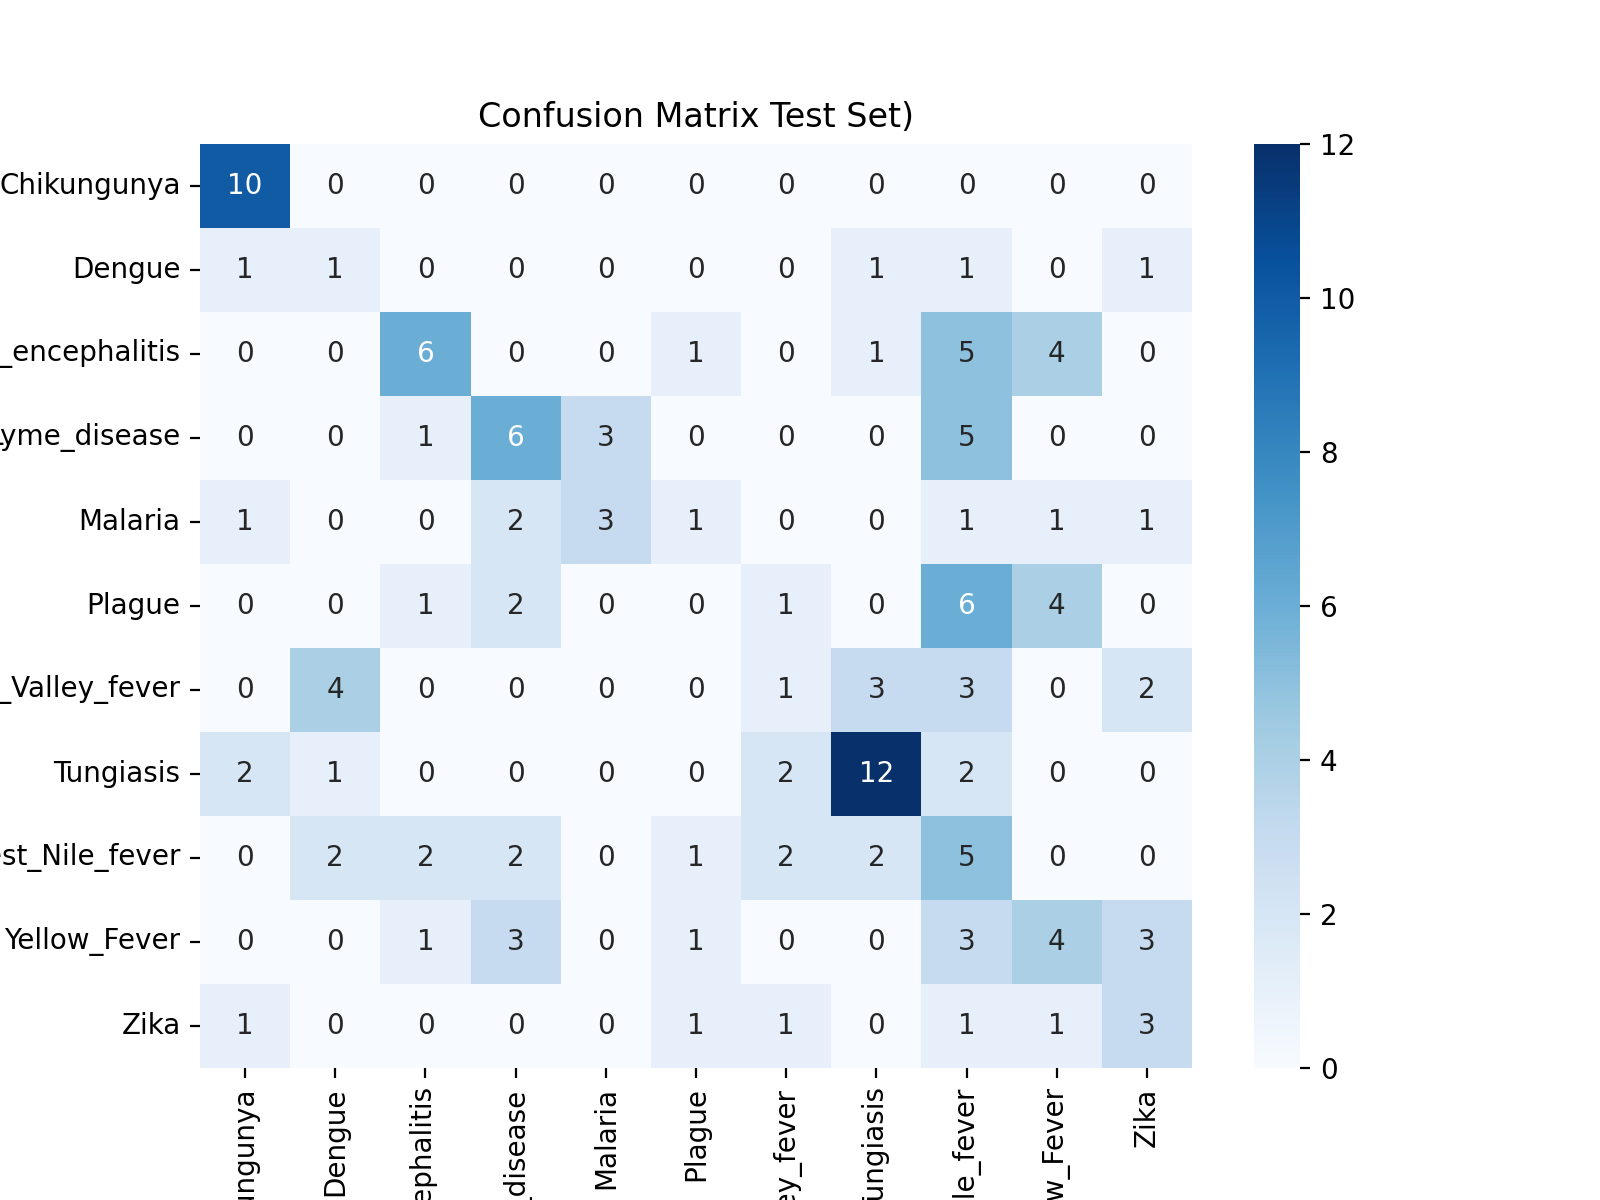
\includegraphics[width=1\linewidth]{Confusion_Matrix_Test_Set.png}
    \caption{Features Correlation Heat Map. Blue areas indicate low correlation.}
    \vspace{-1em} % Reduce vertical spacing
    \end{figure}

\section{Discusion and further analysis}
We will apply a clustering algorithm to determine the optimal number of clusters within the dataset. 
If the clusters are not evenly distributed, or if certain features exhibit high compactness within a cluster,
it may suggest that the dataset lacks sufficient discriminative features to effectively differentiate between distinct patterns."

\subsection{Clustering sympoms pattern}
We will employ the k-means clustering algorithm and expect the k-means plateau to be as high as possible, 
or at least close to the expected value based on the characteristics of our datasete this hypothesis the 
following subsequent analysis is performed:
\begin{figure}[H]  
    \centering
    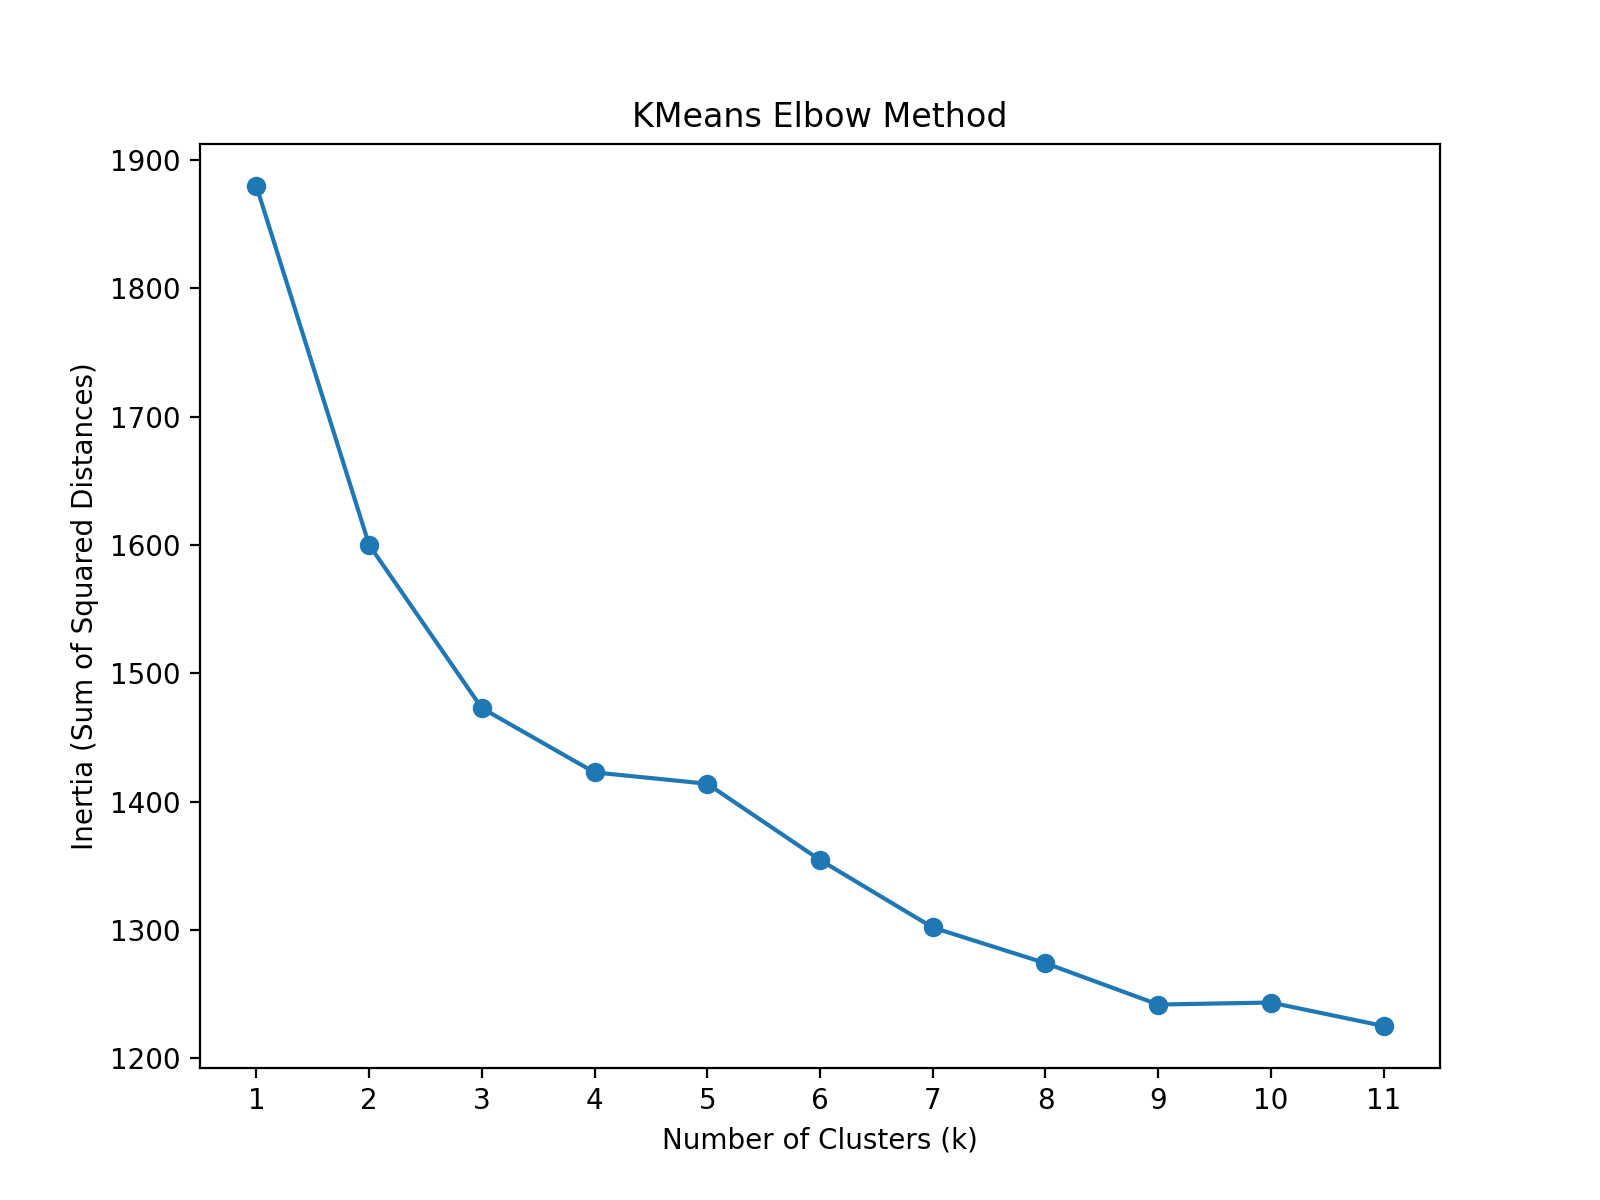
\includegraphics[width=1\linewidth]{Kmeanselbow.png}
    \caption{Features Correlation Heat Map. Blue areas indicate low correlation.}
    \vspace{-1em} % Reduce vertical spacing
    \end{figure}

\subsection{Clustering Results}
The elbow inflection point is found between 4 and 6 clusters. This suggests that most of the points can be effectively grouped within this range. Beyond 6 clusters, diminishing returns occur, 
indicating that the model stared to clump with too few  cluster centers.


\section{Conclusions and Further analysis}
\subsection{Further feature engineering}
Clustering optimal suggests data is hard to separate 
We could start to create features with a cross interaction
machanis between sympoms for example if sympom A and B happen then make another switch
This Aproach could in principle improve our classification, and we could repeat our clustering
analysis to see if the features are enough 
\appendix
\section{Additional tables}

\begin{figure}[H] % Fix the figure at its exact position
    \centering
    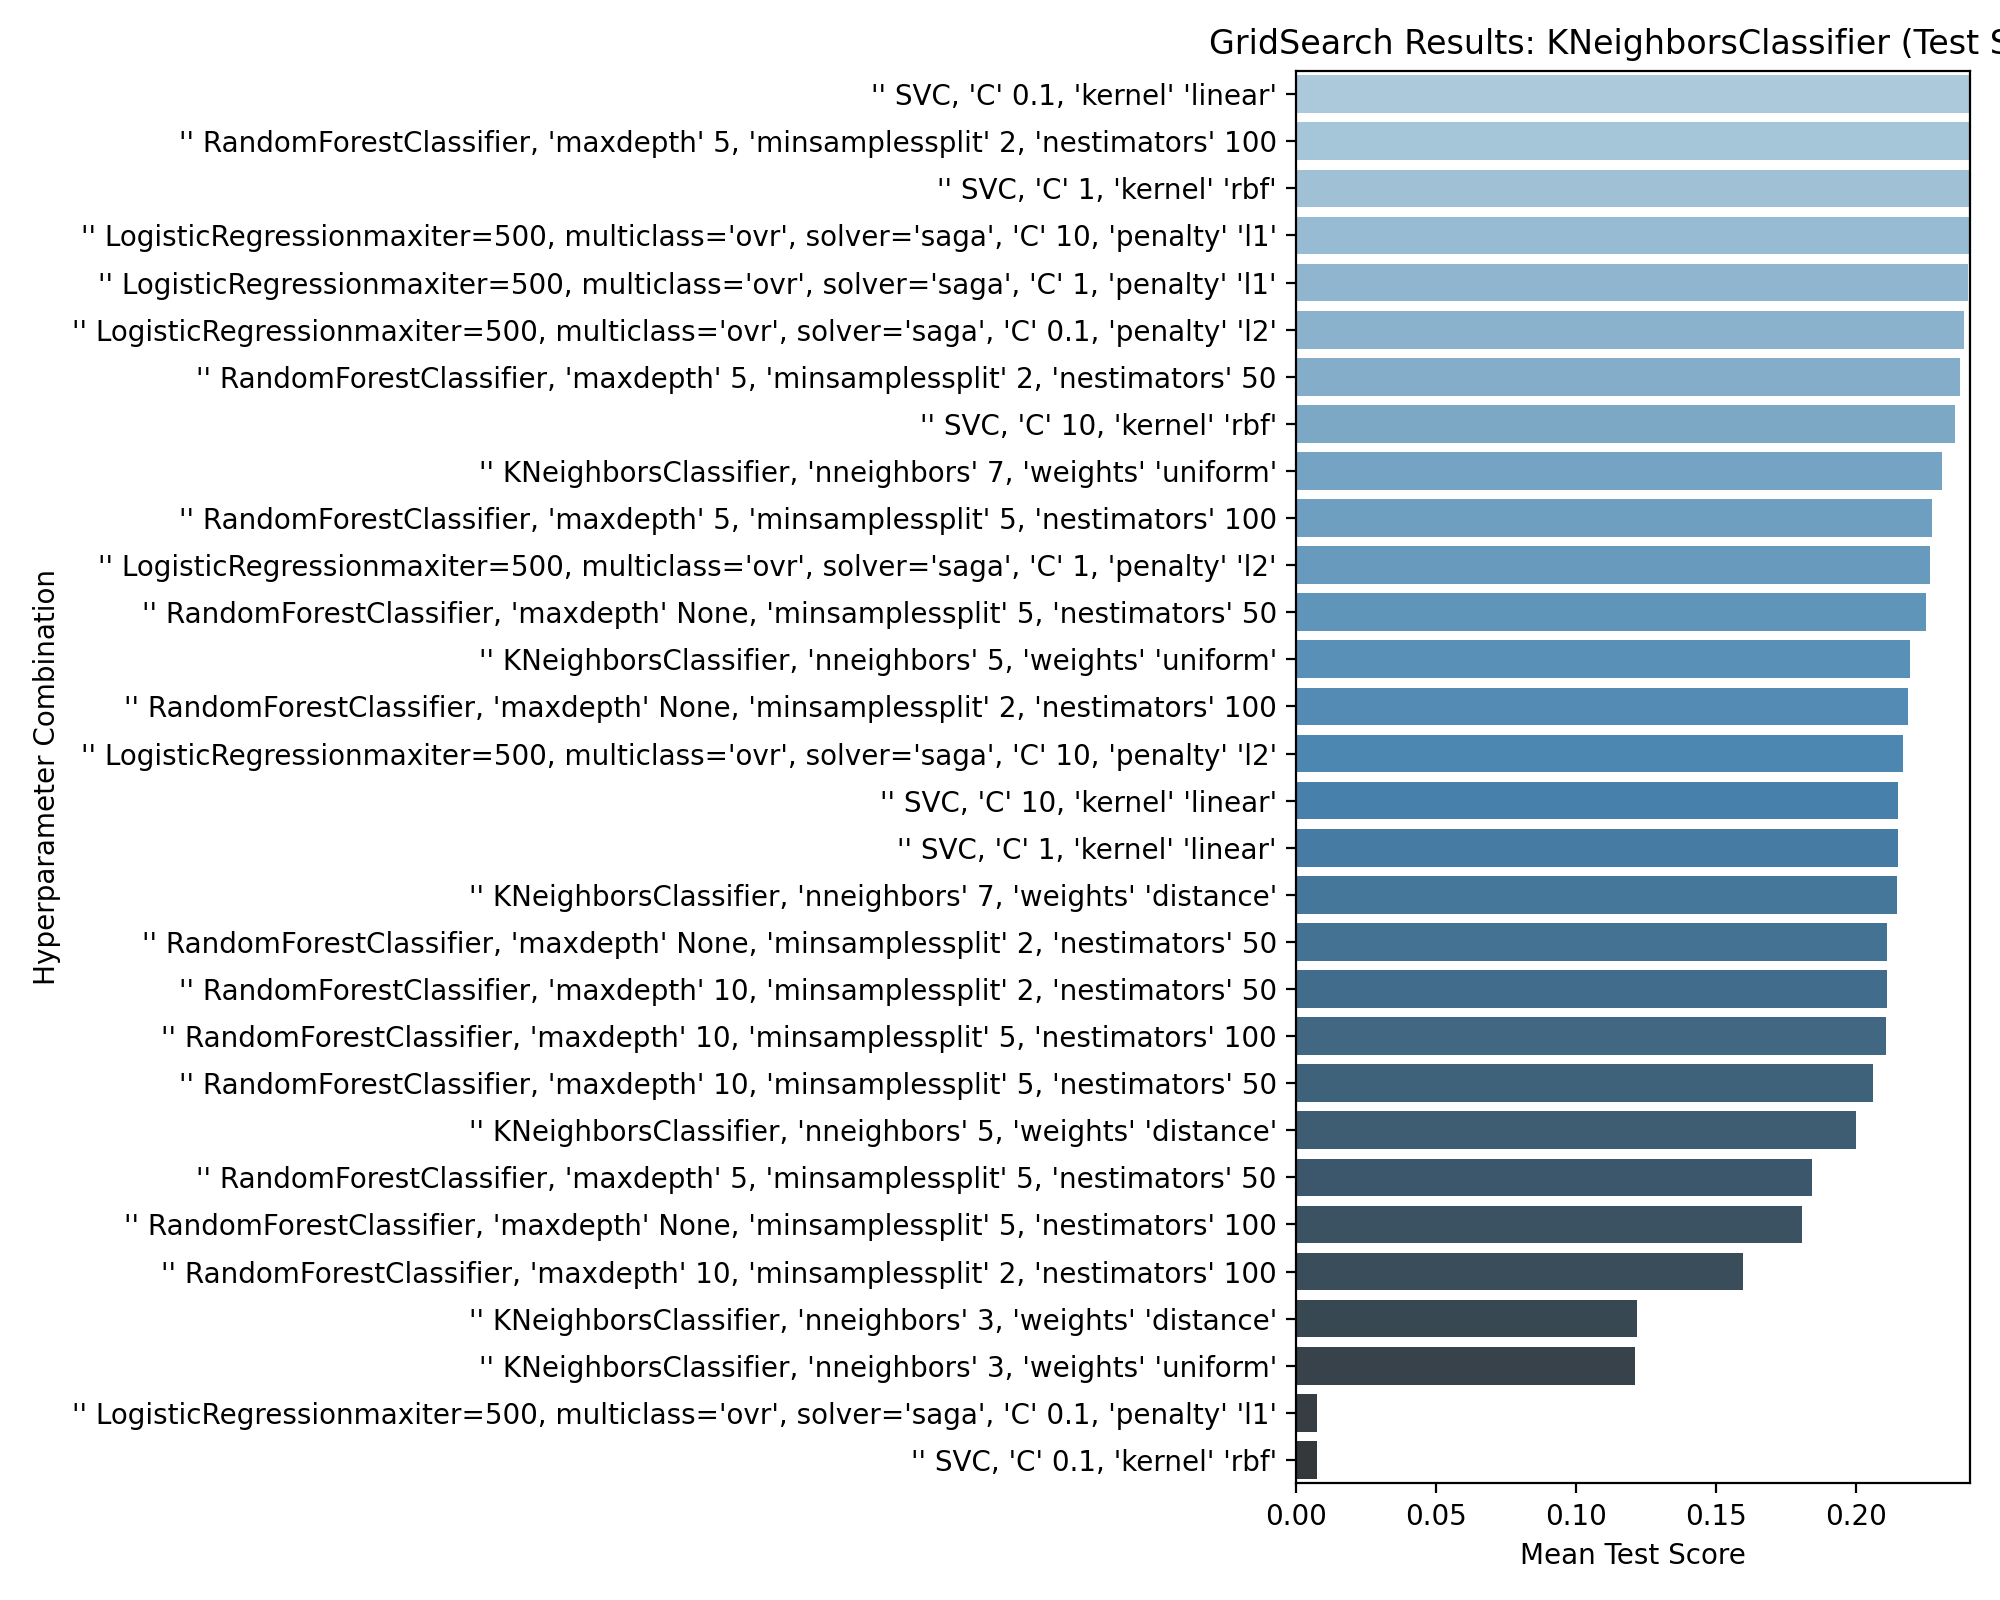
\includegraphics[width=.7
    \linewidth]{TestSet.png}
    \caption{Performace Test Set}
    \label{fig:disease_distribution}
    \vspace{-1em} % Reduce vertical spacing after the figure
\end{figure}

\begin{figure}[H] % Fix the figure at its exact position
    \centering
    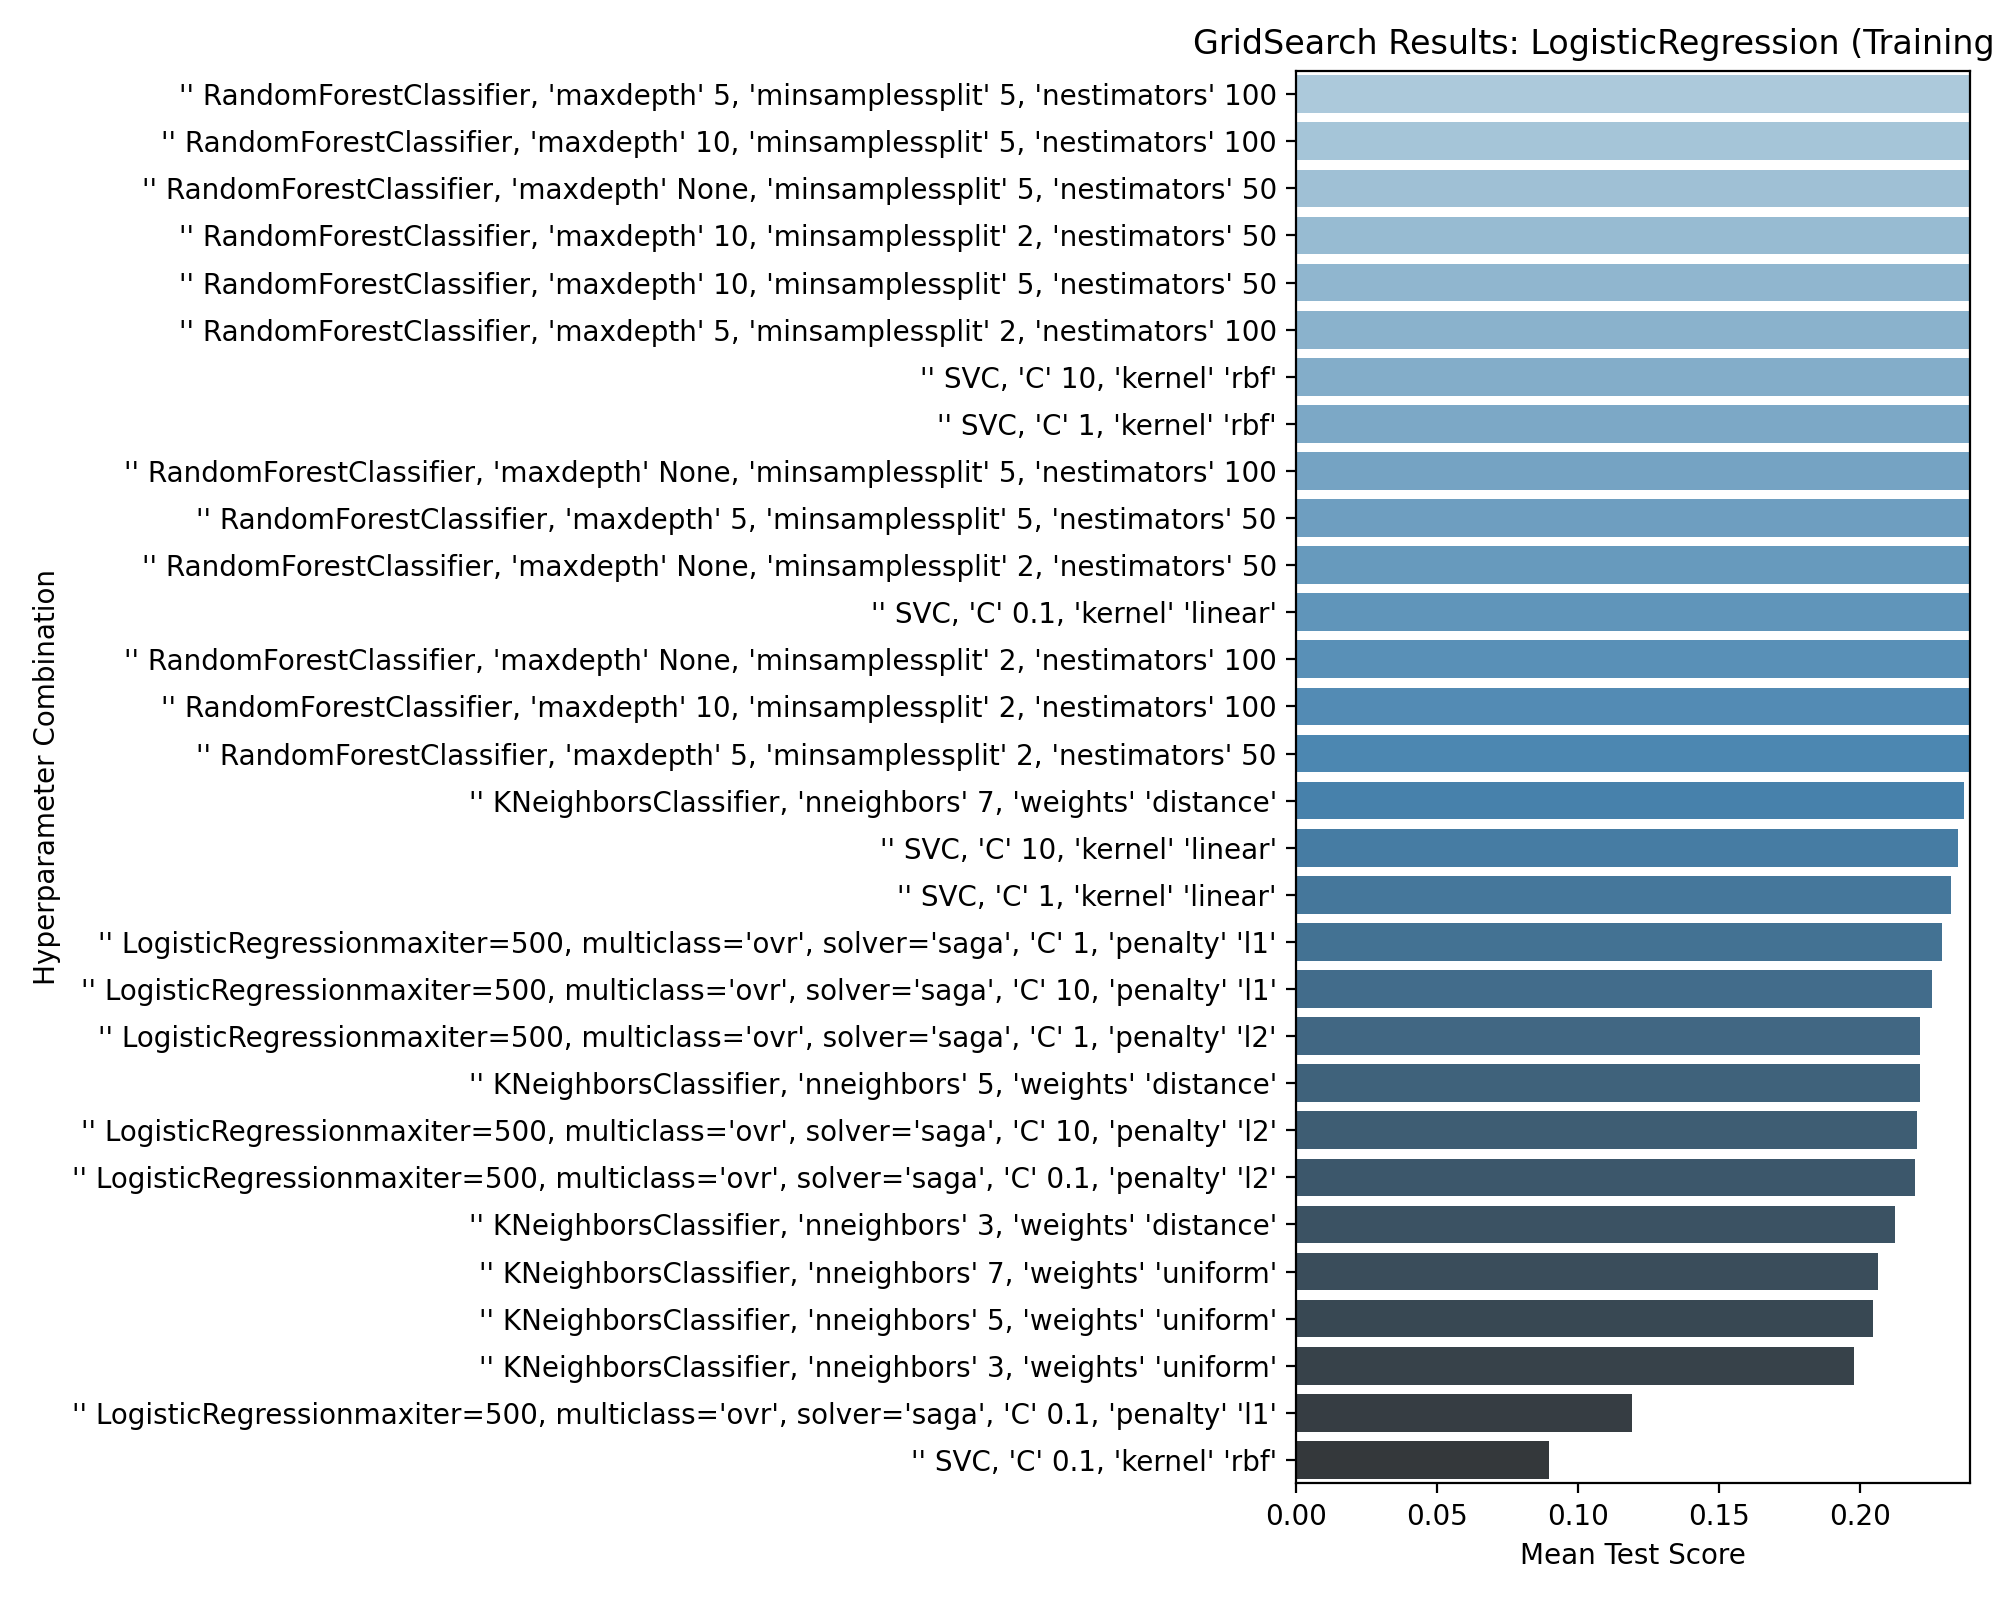
\includegraphics[width=.7
    \linewidth]{TrainingSet.png}
    \caption{Performace Training Set}
    \label{fig:disease_distribution}
    \vspace{-1em} % Reduce vertical spacing after the figure
\end{figure}

\section{Jupyter notebook}
Code used for this analysis \cite{arath2024clustering}.

\label{sec:appendix}
\bibliographystyle{alpha}
\bibliography{references}
\end{document}